\section{Attachements}

\subsection{A1 Tiefpassentwurf mit fir()}


 \lstinputlisting[style=matlab, caption={butterfly correction}, label={lst:butterfly}]{Code/fir_2a.m}

\begin{figure}
\centering
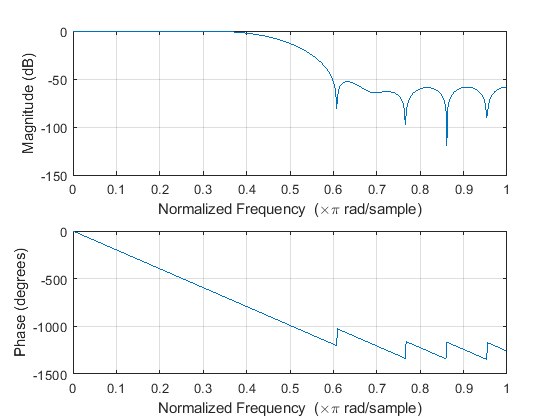
\includegraphics[width=0.7\linewidth]{Bilder/Attachment_A1_fir_2a_Amplitudengang}
\caption{}
\label{fig:Attachment_A1_fir_2a_Amplitudengang}
\end{figure}

\begin{figure}
\centering
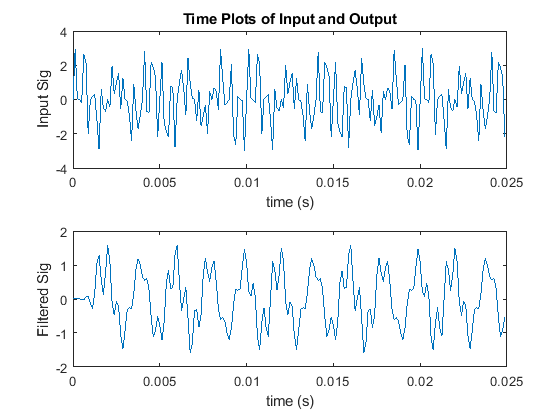
\includegraphics[width=0.7\linewidth]{Bilder/Attachment_A1_fir_2a_Timeplot}
\caption{}
\label{fig:Attachment_A1_fir_2a_Timeplot}
\end{figure}

\begin{figure}
\centering
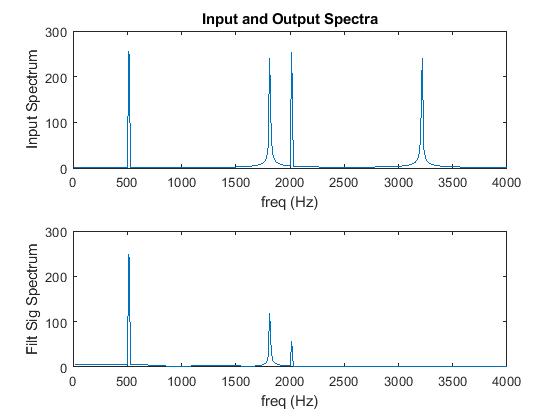
\includegraphics[width=0.7\linewidth]{Bilder/Attachment_A1_fir_2a_Spektrum}
\caption{}
\label{fig:Attachment_A1_fir_2a_Spektrum}
\end{figure}


\newpage
\subsection{A2 Tiefpassentwurd mit firpm()}

\subsection{B Bandpass-Filterentwurf}

\subsection{C1 Analoge Übertragungscharakteristik des DSK Boards}

\subsection{C2 Echtzeit-Festkomma-Impementierung des FIR-Filters}


\subsection{C3 Vergleich des Amplitudengangs vom FIR-Filter Matlab - DSK Board}

\subsection{D Profiling FIR-ISR}

\subsection{E Weichenfilter Transformation mit $h_{TP} \rightarrow h_{HP} .............$}

\subsection{F Weichenfilter Amplitudengang Hoch- und Tiefpass}

\subsection{G Weichenfilter Transformation mit $h_{TP} \rightarrow h_{HP} ..............$}
 
